\documentclass[conference]{IEEEtran}
\IEEEoverridecommandlockouts
\usepackage{cite}
\usepackage{amsmath,amssymb}
\usepackage{graphicx}
\usepackage{textcomp}
\usepackage{booktabs}
\usepackage{url}
\usepackage[caption=false,font=footnotesize]{subfig}
\usepackage{tikz}
\usetikzlibrary{positioning,fit,backgrounds,arrows.meta,calc}

\newcommand{\uV}{\,\textmu V}
\newcommand{\uVrms}{\,\textmu V\textsubscript{rms}}
\newcommand{\uVpp}{\,\textmu V\textsubscript{pp}}
\newcommand{\uA}{\,\textmu A}
\newcommand{\uW}{\,\textmu W}
\newcommand{\um}{\,\textmu m}
\newcommand{\nVrtHz}{\,nV/$\sqrt{\mathrm{Hz}}$}
% Pending results. Every \tbd must be filled or removed before submission.
\newcommand{\tbd}[1]{\textcolor{red}{\textbf{[#1]}}}
% Double-blind review (VLSI-DAT 2026 required it: no names, affiliations or e-mail).
% Confirm in the 2027 call; set \blindtrue for an anonymous submission.
\newif\ifblind
\blindfalse

\begin{document}
\bstctlcite{IEEEexample:BSTcontrol}

\title{Neonatal Seizure Detection with a SKY130 EEG Front End and a Bit-Exact FPGA Detector}

% Add a faculty co-author here only if they contribute to the work or the manuscript.
\ifblind
\author{\IEEEauthorblockN{Anonymous submission}
\IEEEauthorblockA{Author names and affiliations withheld for double-blind review}}
\else
\author{\IEEEauthorblockN{A Sai Chaithr Choudary}
\IEEEauthorblockA{Department of Electronics and Communication Engineering\\
National Institute of Technology Warangal, India\\
chaithr45@gmail.com}}
\fi

\maketitle

\begin{abstract}
Most neonatal seizures have no clinical signs and are found only by continuous EEG review. We present a seizure monitor built from an EEG analog front end (AFE) in the open SKY130 process and a detector in the programmable logic of an AMD Kria KV260. The AFE fits a 1$\times$2 Tiny Tapeout tile; in post-layout simulation it has 37.8\,dB of gain, 2.95\uVrms{} of input noise from 0.5 to 100\,Hz and over 81\,dB of PSRR at 28\uW, and post-layout simulation caught two parasitic couplings that DRC and LVS had passed. The detector scores 108 integer features with 100 gradient-boosted trees trained on the hardware's own integer arithmetic, so the evaluated and the built detector are identical. On the KV260 it matched its golden model in 106,359 of 106,359 values, with a measured worst-case latency of 24\,\textmu s per frame, in 9,592 LUTs and 62 DSP slices. Under nested patient-wise cross-validation on 79 neonates it finds 47.8\% of seizures at 0.91 false alarms per hour; a CNN reference reaches only 49.8\% under the same protocol, at about 300 times the operations. With the post-layout AFE model in the signal path, it finds \tbd{E10-B sensitivity}\% at \tbd{E10-B FA/h} false alarms per hour.
\end{abstract}

\begin{IEEEkeywords}
Neonatal seizure detection, EEG front end, SKY130, FPGA, gradient-boosted trees, bit-exact verification
\end{IEEEkeywords}

\section{Introduction}

In a video-EEG study, only 34\% of 526 electrographic neonatal seizures had clinical signs, and staff recognised 9\%~\cite{murray2008}. Recognition therefore needs continuous EEG read by an expert, which most neonatal units cannot provide around the clock, and machine-learning decision support has reached a randomised trial~\cite{pavel2020}. Neonatal detectors, however, run as workstation software~\cite{temko2011,ansari2019,oshea2020}. Seizure-detection hardware targets adult and paediatric data with patient-specific training~\cite{verma2010,shoaran2018,shin2022,busia2025}, which a newborn cannot provide, and EEG amplifiers are reported by circuit figures of merit~\cite{harrison2003,lee2019,park2022}, not by what a detector needs.

Hardware also opens two gaps between the design that is evaluated and the one that is built. A model trained in floating point and quantised afterwards silently changes decisions, and tuning and testing on the same patients overstates performance~\cite{varma2006}. An amplifier layout that passes DRC and LVS can still differ from its schematic through parasitic coupling. This paper closes both gaps. Its contributions are:
\begin{itemize}
\item a SKY130~\cite{sky130} EEG AFE on a Tiny Tapeout~\cite{tinytapeout} tile, generated as code and verified to post-layout simulation, which found two defects that rule checks cannot see;
\item a neonatal seizure detector in FPGA logic, trained on the hardware's exact integer features and bit-exact from the Python reference to the board;
\item a pre-registered, nested patient-wise evaluation on the public Helsinki dataset~\cite{stevenson2019}, repeated with the AFE model in the signal path.
\end{itemize}
To our knowledge, this is the first neonatal seizure detector in FPGA logic evaluated patient-independently. \ifblind Design files and scripts will be made public after review.\else Design files and scripts are public.\footnote{\url{https://github.com/chaithr45/tt-eeg-afe}}\fi

\begin{figure*}[t]
\centering
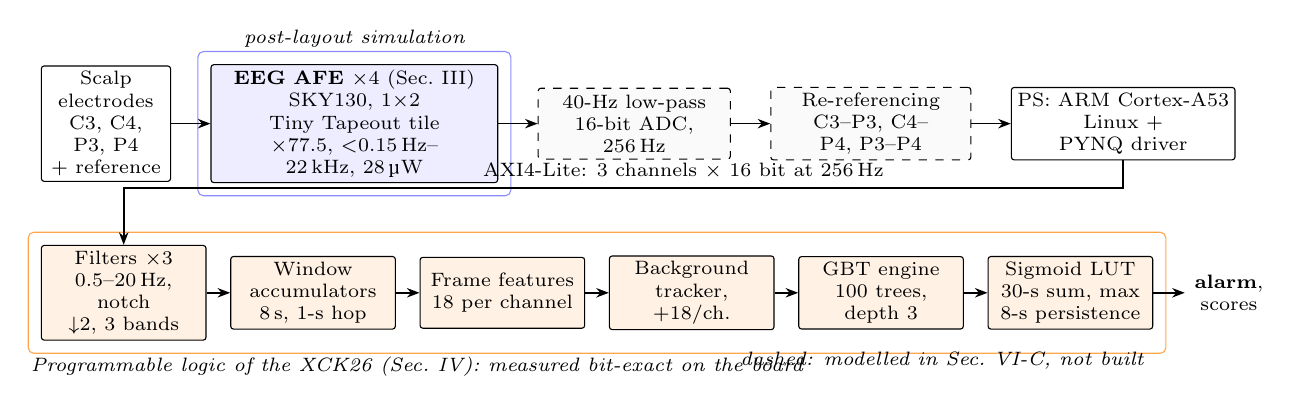
\begin{tikzpicture}[font=\scriptsize, node distance=4mm,
  box/.style={draw, rounded corners=1pt, align=center, inner sep=2pt, minimum height=9mm, fill=white},
  ana/.style={box, fill=blue!7},
  dig/.style={box, fill=orange!10, text width=19.5mm},
  fut/.style={box, dashed, fill=gray!4},
  ar/.style={-{Stealth[length=1.6mm]}, semithick}]
\node[box, text width=15mm] (el) {Scalp electrodes\\C3, C4, P3, P4\\+ reference};
\node[ana, right=5mm of el, text width=35mm] (afe) {\textbf{EEG AFE} $\times$4 (Sec.~III)\\SKY130, 1$\times$2 Tiny Tapeout tile\\$\times$77.5, $<$0.15\,Hz--22\,kHz, 28\uW};
\node[fut, right=5mm of afe, text width=23mm] (adc) {40-Hz low-pass\\16-bit ADC, 256\,Hz};
\node[fut, right=5mm of adc, text width=24mm] (rr) {Re-referencing\\C3--P3, C4--P4, P3--P4};
\node[box, right=5mm of rr, text width=27mm] (ps) {PS: ARM Cortex-A53\\Linux + PYNQ driver};
\node[dig, below=8mm of el.south west, anchor=north west] (f1) {Filters $\times$3\\0.5--20\,Hz, notch\\$\downarrow$2, 3 bands};
\node[dig, right=3mm of f1] (f2) {Window\\accumulators\\8\,s, 1-s hop};
\node[dig, right=3mm of f2] (f3) {Frame features\\18 per channel};
\node[dig, right=3mm of f3] (f4) {Background\\tracker, +18/ch.};
\node[dig, right=3mm of f4] (f5) {GBT engine\\100 trees, depth 3};
\node[dig, right=3mm of f5] (f6) {Sigmoid LUT\\30-s sum, max\\8-s persistence};
\node[right=4mm of f6, align=center] (al) {\textbf{alarm},\\scores};
\draw[ar] (el) -- (afe);
\draw[ar] (afe) -- (adc);
\draw[ar] (adc) -- (rr);
\draw[ar] (rr) -- (ps);
\draw[ar] (ps.south) -- ++(0,-3.5mm) -| node[pos=0.22, above=-0.5pt] {AXI4-Lite: 3 channels $\times$ 16 bit at 256\,Hz} (f1.north);
\foreach \a/\b in {f1/f2, f2/f3, f3/f4, f4/f5, f5/f6, f6/al} \draw[ar] (\a) -- (\b);
\begin{scope}[on background layer]
\node[draw=blue!45, rounded corners=2pt, fit=(afe), inner sep=1.6mm,
      label={[font=\scriptsize\itshape, anchor=south, inner sep=1pt]north:post-layout simulation}] {};
\node[draw=orange!70, rounded corners=2pt, fit=(f1)(f6), inner sep=1.6mm,
      label={[font=\scriptsize\itshape, anchor=north west, inner sep=1pt]south west:Programmable logic of the XCK26 (Sec.~IV): measured bit-exact on the board}] {};
\end{scope}
\node[font=\scriptsize\itshape, anchor=north east] at ($(f6.south east)+(0,-1.6mm)$) {dashed: modelled in Sec.~VI-C, not built};
\end{tikzpicture}
\caption{The monitor: one single-ended AFE per electrode, digital re-referencing and the detector in the programmable logic (PL), fed by the processing system (PS).}
\label{fig:system}
\end{figure*}

\section{System}

Each of four scalp electrodes (Fig.~\ref{fig:system}) is amplified single-ended against a common reference by one AFE; a tile has two analog pins, so each chip carries one channel. The outputs are digitised at 256\,Hz, the rate of the Helsinki recordings, and the detector's bipolar derivations are formed by subtraction. The PS streams them as 16-bit samples to the detector in the PL and reads alarms and scores back.

\section{Analog Front End}

\subsection{Circuit}

The input is AC-coupled through $C_1 = 11.9$\,pF to the inverting input of an operational transconductance amplifier (OTA), with $C_2 = 154$\,fF, a pseudo-resistor and a reset switch in feedback, so the midband gain is $C_1/C_2 = 77.5$\,V/V (Fig.~\ref{fig:sch})~\cite{harrison2003}. The non-inverting input sees $C_1'$ to ground rather than to the signal, so noise on the reference VREF reaches the output with a gain of about 1 instead of 78 and a simple on-chip reference suffices. Each pseudo-resistor is two back-to-back PMOS pairs in series, about $2\times10^{13}\,\Omega$, which places the high-pass corner $f_L$ at 0.04--0.14\,Hz over corners at 37\,\textdegree C. Pseudo-resistors take about 15\,s to settle at power-up, so a 10-ms reset pulse ties their internal nodes and returns the output to within 1\,mV of VREF after a 20-mV artifact.

The OTA is a two-stage Miller design with a 150/8-\textmu m PMOS input pair at 2\uA{} per side. A first version, with short mirror devices, had 22\uVrms{} of noise dominated by the mirror's $1/f$ noise; because that contribution falls roughly as $1/L^2$, each mirror device became three 7/20-\textmu m transistors in series, and a larger $C_1$, which lowers the noise gain set by the 3-pF input capacitance, brought the total to 2.9\uVrms. The open-loop gain is 99\,dB and the loop phase margin 86\textdegree, so the OTA drives the pin and a 15-pF load without a buffer. A subthreshold beta-multiplier and a weak-inversion VREF are on the tile; the whole circuit draws 15.7\uA{} from 1.8\,V.

\begin{figure}[t]
\centering
\subfloat[]{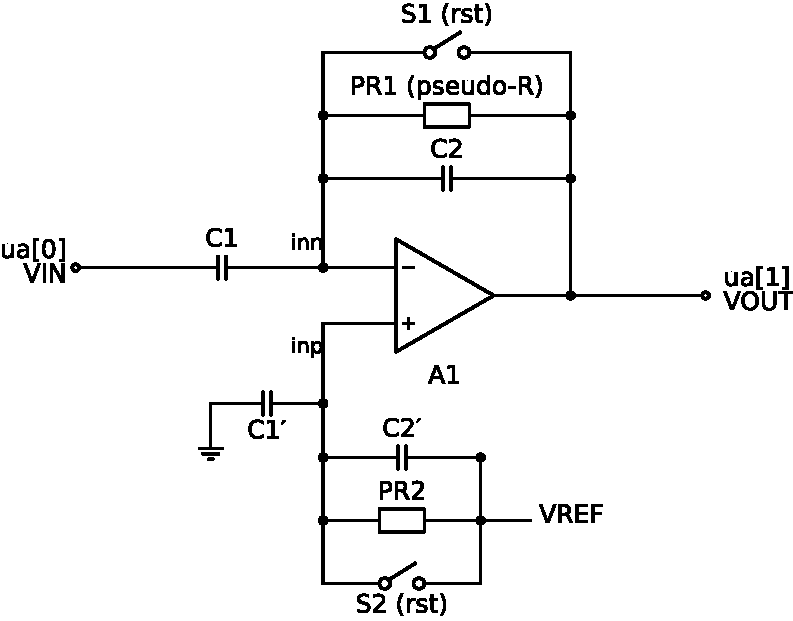
\includegraphics[width=0.72\columnwidth]{figs/afe_top.pdf}}\\[-1mm]
\subfloat[]{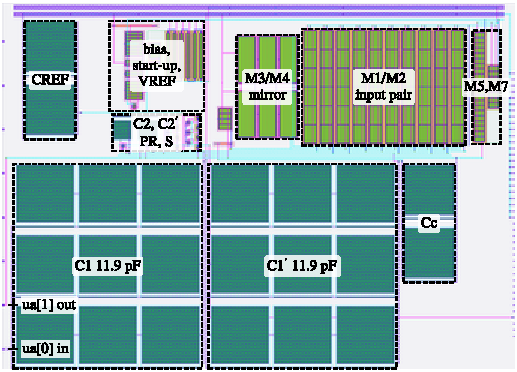
\includegraphics[width=0.86\columnwidth]{figs/layout_annotated.pdf}}
\caption{(a) Capacitive-feedback amplifier: $C_1 = C_1' = 11.9$\,pF, $C_2 = C_2' = 154$\,fF; PR, pseudo-resistor; S1, S2, reset switches. (b) Layout of the 161$\times$226-\textmu m tile, rotated 90\textdegree{} and generated by Python scripts that drive Magic; $C_c$ and CREF are 2-pF MIM capacitors.}
\label{fig:sch}
\end{figure}

\subsection{Layout and Post-Layout Verification}

One build script regenerates the layout from code, runs Magic DRC and Netgen LVS on the core and the tile, and extracts parasitics~\cite{edatools}; the tile passes the Tiny Tapeout precheck locally and in continuous integration. The extracted core is simulated against the schematic with the on-chip bias, a model of the shuttle's analog pin path and a 15\,pF\,$\parallel$\,1\,M$\Omega$ load. The first complete layout passed every rule check, but post-layout simulation showed 0.56\,dB of excess gain, caused by 12\,fF between the output and the non-inverting input, and a 50-Hz PSRR of 77 instead of 96\,dB, caused by 1.35\,fF from the supply and bias lines onto the inverting input. A ground shield track removed the gain error, and 1.5\um{} more spacing with a metal-1 line on the tail node raised the PSRR to 85.6\,dB. Neither defect broke a rule or changed connectivity, so only extraction and simulation could find them.

\begin{table}[t]
\caption{AFE Post-Layout Results and Comparison}
\label{tab:afe}
\centering
\footnotesize
\setlength{\tabcolsep}{2.4pt}
\begin{tabular}{@{}lcccc@{}}
\toprule
 & This work & \cite{harrison2003} & \cite{lee2019} & \cite{park2022} \\
\midrule
Process & SKY130 & 1.5\um{} & 65\,nm & 110\,nm \\
Supply (V) & 1.8 & 5 & 0.8 & 1/1.5 \\
Chopper & no & no & yes & yes \\
Gain (dB) & 37.8 & 39.5 & -- & -- \\
Noise (\textmu V\textsubscript{rms}) & 2.95\textsuperscript{a} & 2.2 & 0.38\textsuperscript{a} & 0.36\textsuperscript{b} \\
Power (\textmu W) & 28\textsuperscript{c} & 80 & 4.5 & 3.8 \\
NEF & $\approx$10 & 4.0 & 3.32 & 1.54 \\
PSRR at 50\,Hz (dB) & $>$81\textsuperscript{d} & -- & -- & -- \\
Area (mm$^2$) & 0.036\textsuperscript{e} & 0.16 & -- & -- \\
Result & post-layout & measured & measured & measured \\
\bottomrule
\multicolumn{5}{@{}p{0.98\columnwidth}@{}}{\scriptsize \textsuperscript{a}0.5--100\,Hz. \textsuperscript{b}0.5--300\,Hz. \textsuperscript{c}Bias and VREF included. \textsuperscript{d}All corners. \textsuperscript{e}Whole 1$\times$2 tile.}
\end{tabular}
\end{table}

Parasitics change the final gain by $-0.04$\,dB and the in-band noise by $+0.02$\uVrms{} at every simulated corner and with both SKY130 model sets (Table~\ref{tab:afe}). The noise is dominated by $1/f$ noise (390\nVrtHz{} at 10\,Hz against a 48-nV/$\sqrt{\mathrm{Hz}}$ floor). In 200 Monte Carlo samples the gain spread is $\sigma = 0.06$\%. The NEF of about 10 is high because only 4 of the 15.7\uA{} flow in the input pair; the chopper designs of~\cite{lee2019,park2022} are nearly an order of magnitude quieter, and chopping is the path to closing that gap.

\section{Seizure Detector}

\subsection{Data and Evaluation Protocol}

The Helsinki dataset~\cite{stevenson2019} holds EEG from 79 term neonates (111.9\,h) at 256\,Hz, annotated by three experts; the majority gives 492 seizures in 46 neonates. We use C3--P3, C4--P4 and P3--P4. All results use nested patient-wise cross-validation: five outer folds of neonates are each tested once, and every choice of features, model and threshold is made by cross-validation inside the training neonates, with the threshold set for 1 false alarm per hour (FA/h) on inner out-of-fold scores. Success criteria were committed before any result was computed. We report event sensitivity, FA/h, AUC and Cohen's $\kappa$~\cite{cohen1960}, with 95\% confidence intervals from resampling neonates.

\subsection{Features and Hardware-Exact Training}

Ten second-order sections per channel give a 0.5--20-Hz band, a 50-Hz notch and three sub-bands. Every second, 18 features are computed over the last 8\,s, among them line length~\cite{esteller2001}, band energies, a spectral entropy from the band energies and Hjorth parameters, each paired with a version normalised to a running per-channel background: 36 per channel, 108 in all. Windows are formed from eight 1-s partial sums, so an 8-s window costs eight accumulators instead of 1,024 stored samples, and no feature needs a divider.

A gradient-boosted tree ensemble~\cite{friedman2001} (100 trees, depth 3) scores each channel; the alarm is raised when the maximum over channels of a 30-s sum of sigmoid outputs stays above a threshold for 8\,s. Quantising a floating-point ensemble after training cannot be made exact: at Q16, 401 of 500,000 node comparisons took a different branch, because some feature values lay within $10^{-12}$ of a split. We therefore define the features in the RTL's integer arithmetic and train on these integers, so every split is an integer comparison the hardware makes exactly. Against training on floating-point features, all paired differences include zero (pooled AUC $+0.001$ [$-0.004$, $+0.005$]; sensitivity $0.0$ [$-1.1$, $+1.2$] points), so exactness cost no measurable accuracy.

\subsection{Architecture}

The detector is an AXI4-Lite peripheral at 100\,MHz. Between two samples there are 390,625 cycles, so arithmetic units are shared and sequenced and state lives in RAM: once per second the features, background tracker and tree engine run for each channel in turn, 2,399 cycles in the worst case. The tree engine holds the model in two 1,500-word RAMs written over AXI, so a retrained model needs no new bitstream, and uses 162 LUTs.

\section{Verification and Measurement}

Both halves are checked against one reference each (Table~\ref{tab:verif}). The AFE's reference is its schematic; the detector's is a Python golden model that follows the RTL's operation order, and any difference counts as a defect. On the KV260, a PYNQ driver streamed 300\,s of EEG from each of three neonates; all 106,359 values (every feature, tree output, score and decision state) matched, and the 1,500 model words read back unchanged. These neonates were in the training set, so this run establishes correctness, not accuracy. The busy-cycle counter read a maximum of 2,399 cycles over a full 62-min recording, equal to simulation.

\begin{table}[t]
\caption{Verification and On-Board Measurement}
\label{tab:verif}
\centering
\footnotesize
\setlength{\tabcolsep}{3pt}
\begin{tabular}{@{}lll@{}}
\toprule
Check & Reference & Result \\
\midrule
\multicolumn{3}{@{}l}{\emph{AFE (SKY130)}}\\
DRC, LVS, core and tile & rules, schematic & 0 errors, match \\
Tiny Tapeout precheck & shuttle rules & pass (local, CI) \\
Post-layout simulation & schematic & $-0.04$\,dB, $+0.02$\uVrms \\
\midrule
\multicolumn{3}{@{}l}{\emph{Detector}}\\
Blocks and core (xsim) & golden model & 2.66\,M values, 0 diff. \\
AXI, 62-min record (xsim) & golden model & 453,739 reads, 0 diff. \\
KV260, 3 neonates (board) & golden model & 106,359 values, 0 diff. \\
KV260, worst-case latency & simulation & 2,399 cycles, equal \\
\bottomrule
\end{tabular}
\end{table}

\section{Results}

\subsection{Detection}

Table~\ref{tab:det} compares detectors scored on the same folds. The built detector finds 47.8\% of seizures (95\% CI 34.5--60.4\%) at 0.91\,FA/h and at least one seizure in 33 of 46 neonates. The CNN reference has the highest AUC but only 2 points more event sensitivity, at about 300 times more operations per second, and the RBF SVM's support vectors exceed the device's block RAM in three of five folds.

\begin{table}[t]
\caption{Detectors on Identical Nested Folds (1\,FA/h Target)}
\label{tab:det}
\centering
\footnotesize
\setlength{\tabcolsep}{2.1pt}
\begin{tabular}{@{}lcccc@{}}
\toprule
 & Pooled & Sens.\ \% & Neonates & \\
Detector & AUC & (FA/h) & detected & $\kappa$ \\
\midrule
Threshold rule & 0.700 & 26.6 (1.22) & 11/46 & 0.220 \\
RBF SVM & 0.837 & 44.3 (0.91) & 31/46 & 0.375 \\
CNN on raw EEG (reference) & 0.888 & 49.8 (1.10) & 39/46 & 0.573 \\
\textbf{Hardware-exact trees (built)} & \textbf{0.816} & \textbf{47.8 (0.91)} & \textbf{33/46} & \textbf{0.422} \\
\midrule
\multicolumn{5}{@{}l}{\emph{Built detector behind the AFE model (Sec.~VI-C)}}\\
AFE, 40-Hz low-pass, 16-bit ADC & \tbd{TBD} & \tbd{TBD} & \tbd{TBD} & \tbd{TBD} \\
AFE, no anti-alias filter & \tbd{TBD} & \tbd{TBD} & \tbd{TBD} & \tbd{TBD} \\
AFE, $f_L$ 0.04 vs 0.14\,Hz & \tbd{TBD} & \tbd{TBD} & \tbd{TBD} & \tbd{TBD} \\
\bottomrule
\end{tabular}
\end{table}

\subsection{Implementation}

After place and route (xck26-sfvc784-2LV-c) the detector uses 9,592 LUTs (8.2\%), 10,494 flip-flops, 62 DSP slices (5.0\%, 60 of them in the filters) and four 36-Kb block RAMs, and meets timing at 100\,MHz; its worst case is 0.61\% of the cycle budget. Vivado estimates 53\,mW for the detector logic; measured board power rose from 3.10 to 3.42\,W while streaming, a figure that includes the processor feeding the samples. The same integer detector in C on one Cortex-A53 core needs \tbd{E11: median / max time per frame} per frame. Table~\ref{tab:hw} places the design among seizure-detection hardware; of these designs it is the only one evaluated across patients and the only one for neonates.

\begin{table}[t]
\caption{Comparison with Seizure-Detection Hardware}
\label{tab:hw}
\centering
\footnotesize
\setlength{\tabcolsep}{2pt}
\begin{tabular}{@{}lcccc@{}}
\toprule
 & \cite{shoaran2018} & \cite{shin2022} & \cite{busia2025} & This work \\
\midrule
Platform & 65-nm ASIC & 65-nm ASIC & iCE40 FPGA & KV260 FPGA \\
Classifier & GBT & oblique tree & SNN & GBT \\
Patients & iEEG & paed.\ EEG & paed.\ EEG & neonates \\
 & 26 & 24 & 9 & 79 \\
Protocol & per patient & per patient & per patient & \textbf{across patients} \\
Result & F1 87.9\% & sens.\ 95.6\% & 100\% events & 47.8\% at \\
 & & spec.\ 96.8\% & 0.3 FP/h & 0.91 FA/h \\
Power or & 41.2 & 0.227 & 9.1\,mW & 53\,mW \\
energy & nJ/class & \textmu J/class & (meas.) & (est.) \\
Latency & 1.1\,s\textsuperscript{a} & -- & 0.5\,\textmu s & 24\,\textmu s \\
\bottomrule
\multicolumn{5}{@{}p{0.98\columnwidth}@{}}{\scriptsize Per-patient models are trained and tested on the same patient and are not directly comparable with across-patient results. \textsuperscript{a}Delay from seizure onset to detection; the other latencies are processing times per inference or frame.}
\end{tabular}
\end{table}

\subsection{AFE in the Signal Path}

To join the halves, the electrode signals of every recording were passed through the post-layout AFE model before re-referencing: its gain and high-pass response, its input-referred noise spectrum folded into the 0--128-Hz band by sampling at 256\,Hz, an optional single-pole 40-Hz anti-alias filter and a 16-bit converter. The detector, its fold models and thresholds were unchanged. The recordings already contain the clinical amplifier's noise, so the AFE's noise adds to it. With the anti-alias filter the bipolar derivations carry \tbd{E10: 0.5--20 Hz noise} of AFE noise and the built detector finds \tbd{E10-B}\% of seizures at \tbd{FA/h} FA/h (Table~\ref{tab:det}). \tbd{One sentence on what the no-filter and $f_L$-mismatch rows show.}

\section{Limitations and Conclusion}

The AFE is pre-silicon: pseudo-resistors are poorly modelled and may differ by an order of magnitude on silicon, and the AFE is specified for 0--50\,\textdegree C. The converter and re-referencing are modelled, not built. The detector is not at expert level: its $\kappa$ of 0.42 is below the experts' 0.76, and 13 of the 46 neonates with seizures have none detected. The configuration was fixed after the model search on hardware-cost grounds, which we disclose as a protocol amendment; the pre-declared trees-only procedure scored 50.2\%.

A SKY130 EEG front end fits a Tiny Tapeout tile at 2.95\uVrms{} and 28\uW{} in post-layout simulation, and a neonatal seizure detector trained on its own integer arithmetic runs bit-exactly on an FPGA SoC in under 9\% of its logic and 24\,\textmu s per frame. Evaluated across patients and with the front end in the loop, the system shows that the AFE's $1/f$ noise, not the detector's arithmetic, is the next limit to remove.

\section*{Acknowledgment}

\ifblind An AI assistant (Claude, Anthropic) was used\else The author used an AI assistant (Claude, Anthropic)\fi{} for simulation and layout scripting, software development and manuscript drafting. All reported results come from the project repositories and their simulation, evaluation and board logs.

\bibliographystyle{IEEEtran}
\bibliography{refs}

\end{document}
